\documentclass[tikz,border=10pt]{standalone}
\usepackage{pgfplots}
\pgfplotsset{compat=1.18}
\usetikzlibrary{arrows.meta}

\begin{document}
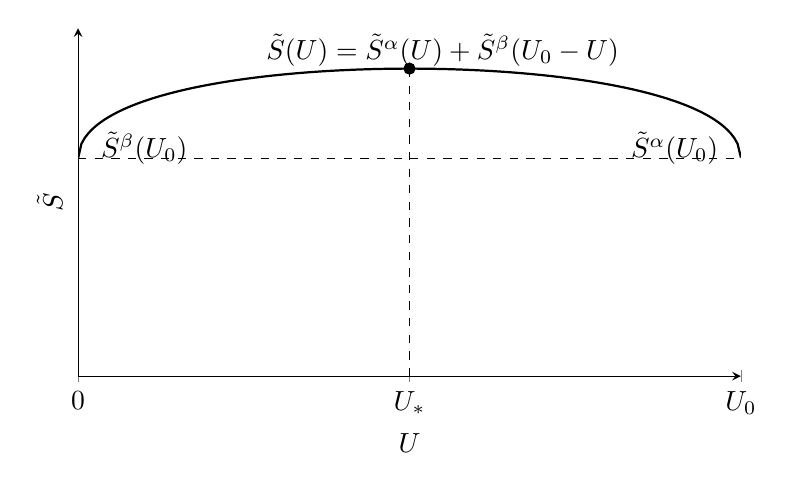
\begin{tikzpicture}
\begin{axis}[
    width=10cm,
    height=6cm,
    xmin=0, xmax=1,
    ymin=0, ymax=1.6,
    xlabel={$U$},
    ylabel={$\tilde{S}$},
    axis lines=left,
    xtick={0,0.5,1},
    xticklabels={$0$,$U_*$,$U_0$},
    ytick=\empty
]
    % Combined entropy curve
    \addplot[black,thick,domain=0:1,samples=200] {sqrt(x)+sqrt(1-x)};

    % Dashed chord line
    \addplot[black,dashed,domain=0:1] {1};

    % Mark maximum point
    \addplot[only marks,mark=*,black] coordinates {(0.5,1.4142)};
    \draw[dashed] (axis cs:0.5,0) -- (axis cs:0.5,1.4142);

    \node at (axis cs:0.55,1.5) {$\tilde{S}(U)=\tilde{S}^\alpha(U)+\tilde{S}^\beta(U_0-U)$};
    \node at (axis cs:0.9,1.05) {$\tilde{S}^\alpha(U_0)$};
    \node at (axis cs:0.1,1.05) {$\tilde{S}^\beta(U_0)$};
\end{axis}
\end{tikzpicture}
\end{document}
